% IR2 experiments. Numbers from report/data/ir2_results.json (Colab T4, run 2, Nov 19) and, for the first
% attempt at idea 3, report/data/run1/ir2_results.json (run 1, same day). Tables: generated/ir2_tables.tex.
\section{Experiments}
\label{sec:exp}

% generated by report/ir2_tables.py, do not edit
\begin{table}[t]
\caption{Idea 1: building the donor layout. Host is the IR1 NumPy/SciPy code on one core, GPU is the same arrays built with CuPy and cuSPARSE (median of 5, synchronised, large from run 3). Identical: all four arrays equal the host ones bit for bit.}
\label{tab:layout}
\small
\begin{tabular}{@{}lrrrc@{}}
\toprule
Size (nnz) & Host ms & GPU ms & Speedup & Identical \\
\midrule
small (3.2 M) & 111.7 & 8.86 & 13$\times$ & yes \\
medium (16.0 M) & 657.0 & 43.02 & 15$\times$ & yes \\
large (76.8 M) & 2,636.9 & 194.42 & 14$\times$ & yes \\
\bottomrule
\end{tabular}
\end{table}

\begin{table*}[t]
\caption{Kernel time in ms (CUDA events, median of 3 trials of 10, or 8 trials for large from run 3, includes the row normalisation) and speedup over the IR1 gather kernel. Max relative error is against the float64 reference after normalisation. 128-thread blocks.}
\label{tab:kernels}
\small
\begin{tabular}{@{}lrrrrrrr@{}}
\toprule
Kernel & \multicolumn{2}{c}{small (3.2 M nnz)} & \multicolumn{2}{c}{medium (16.0 M nnz)} & \multicolumn{2}{c}{large (76.8 M nnz)} & Max rel.\ err \\
 & ms & vs gather & ms & vs gather & ms & vs gather & \\
\midrule
scatter (IR1 v1) & 3.08 & 0.23$\times$ & 25.08 & 0.07$\times$ & 242.4 & 0.02$\times$ & 1.2e-06 \\
gather (IR1 v2) & 0.71 & 1.00$\times$ & 1.72 & 1.00$\times$ & 5.96 & 1.00$\times$ & 2.2e-07 \\
gather\_xr (3b) & 0.42 & 1.68$\times$ & 1.31 & 1.32$\times$ & 6.70 & 0.89$\times$ & 2.2e-07 \\
gather\_fm (3) & 0.39 & 1.84$\times$ & 1.22 & 1.42$\times$ & 4.91 & 1.21$\times$ & 2.2e-07 \\
gather\_cs (2) & 0.82 & 0.87$\times$ & 3.37 & 0.51$\times$ & 10.37 & 0.58$\times$ & 1.2e-06 \\
cuSPARSE SpGEMM & 81.06 & 0.01$\times$ & 323.9 & 0.01$\times$ & -- & -- & 2.8e-07 \\
\bottomrule
\end{tabular}
\end{table*}

\begin{table}[t]
\caption{Idea 2, counted on the host from the actual layouts: adds per nonzero, and lane steps per warp loop iteration (the warp waits for its slowest lane).}
\label{tab:work}
\small
\begin{tabular}{@{}lrrr@{}}
\toprule
 & small & medium & large \\
\midrule
Set bits per cell (no flip) & 19.1 & 19.5 & 19.7 \\
Set bits after the flip & 9.07 & 8.72 & 8.66 \\
Flipped pseudo-bulks (of 900) & 648 & 643 & 645 \\
Adds per nonzero, gather & 32 & 32 & 32 \\
Adds per nonzero, gather\_cs & 10.07 & 9.72 & 9.66 \\
Warp-max set bits per step & 13.84 & 13.46 & 13.56 \\
Lane-step ratio gather / cs & 2.16$\times$ & 2.21$\times$ & 2.20$\times$ \\
\bottomrule
\end{tabular}
\end{table}

\begin{table}[t]
\caption{End to end on the medium instance, ms (median of 5). Host prep is the IR1 layout build or, for the GPU paths, the donor codes. GPU layout includes the fused-mask gather.}
\label{tab:e2e-medium}
\small
\begin{tabular}{@{}lrrrrrr@{}}
\toprule
Path & Host & H2D & Layout & Kernel & D2H & Total \\
\midrule
scatter & 0.0 & 31.6 & 0.0 & 25.3 & 3.6 & \textbf{61.6} \\
gather, host layout (IR1) & 631.7 & 31.9 & 0.0 & 3.2 & 3.3 & \textbf{669.9} \\
gather, GPU layout & 30.9 & 56.1 & 37.8 & 1.7 & 3.3 & \textbf{129.4} \\
gather\_fm, GPU layout & 32.1 & 57.0 & 37.5 & 1.1 & 3.4 & \textbf{130.0} \\
\bottomrule
\end{tabular}
\end{table}

\begin{table}[t]
\caption{End to end on the large instance, ms (median of 5). Host prep is the IR1 layout build or, for the GPU paths, the donor codes. GPU layout includes the fused-mask gather.}
\label{tab:e2e-large}
\small
\begin{tabular}{@{}lrrrrrr@{}}
\toprule
Path & Host & H2D & Layout & Kernel & D2H & Total \\
\midrule
scatter & 0.0 & 147.5 & 0.0 & 242.8 & 6.7 & \textbf{397.1} \\
gather, host layout (IR1) & 2,415.8 & 149.0 & 0.0 & 8.1 & 6.9 & \textbf{2,580.1} \\
gather, GPU layout & 90.4 & 271.1 & 195.2 & 4.8 & 6.8 & \textbf{570.1} \\
gather\_fm, GPU layout & 85.3 & 273.1 & 197.9 & 4.3 & 6.5 & \textbf{566.9} \\
\bottomrule
\end{tabular}
\end{table}

\begin{table}[t]
\caption{Nsight Compute, medium instance, one launch each (SM clock locked at 585 MHz by Nsight, so durations exceed the event timings).}
\label{tab:ncu2}
\footnotesize
\setlength{\tabcolsep}{3pt}
\begin{tabular}{@{}lrrrr@{}}
\toprule
Metric & gather & gather\_xr & gather\_fm & gather\_cs \\
\midrule
Duration (us) & 2,726 & 1,454 & 1,135 & 4,712 \\
SM throughput (\%) & 76.1 & 57.4 & 72.6 & 44.4 \\
L1/TEX throughput (\%) & 86.0 & 74.7 & 69.7 & 89.3 \\
DRAM throughput (\%) & 29.9 & 55.4 & 69.5 & 17.2 \\
Instructions (M) & 160.7 & 79.9 & 78.7 & 110.1 \\
Active threads per instr. & 22.4 & 29.7 & 29.7 & 21.0 \\
Warp cycles per issue & 10.9 & 10.9 & 8.6 & 11.0 \\
Registers per thread & 65 & 65 & 65 & 23 \\
Achieved occupancy (\%) & 84.0 & 79.1 & 79.2 & 33.8 \\
Shared bank conflicts (M) & 0.00 & 0.00 & 0.00 & 21.59 \\
L1/TEX bytes (MB) & 656 & 666 & 269 & 272 \\
DRAM bytes read (MB) & 241 & 238 & 232 & 240 \\
\bottomrule
\end{tabular}
\end{table}

\begin{table}[t]
\caption{Nsight Compute, large (run 3) instance, one launch each (SM clock locked at 585 MHz by Nsight, so durations exceed the event timings).}
\label{tab:ncu-large}
\footnotesize
\setlength{\tabcolsep}{3pt}
\begin{tabular}{@{}lrrrr@{}}
\toprule
Metric & gather & gather\_xr & gather\_fm & gather\_cs \\
\midrule
Duration (us) & 7,494 & 5,391 & 4,106 & 19,170 \\
SM throughput (\%) & 63.8 & 56.6 & 73.1 & 40.6 \\
L1/TEX throughput (\%) & 77.8 & 63.6 & 47.4 & 89.5 \\
DRAM throughput (\%) & 45.5 & 63.2 & 82.2 & 17.8 \\
Instructions (M) & 447.0 & 285.5 & 280.2 & 442.2 \\
Active threads per instr. & 25.1 & 30.7 & 30.7 & 20.6 \\
Warp cycles per issue & 10.5 & 11.5 & 8.9 & 11.2 \\
Registers per thread & 65 & 65 & 65 & 23 \\
Achieved occupancy (\%) & 84.1 & 81.7 & 81.7 & 34.5 \\
Shared bank conflicts (M) & 0.00 & 0.00 & 0.00 & 101.36 \\
L1/TEX bytes (MB) & 2,830 & 2,862 & 914 & 911 \\
DRAM bytes read (MB) & 1,053 & 1,053 & 1,039 & 1,054 \\
\bottomrule
\end{tabular}
\end{table}

\begin{figure}[t]
\centering
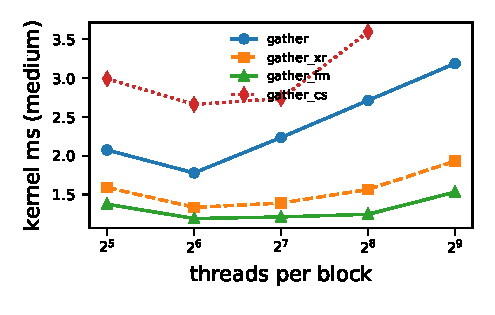
\includegraphics[width=\columnwidth]{figures/ir2_blocks.pdf}
\caption{Block-size sweep on the medium instance (median of 10). gather\_cs stops at 256 threads, where its shared memory reaches 33 KB per block.}
\label{fig:blocks}
\end{figure}



\subsection{Setup}

One Colab session on a Tesla T4 (40 SMs, 320 GB/s, CUDA through CuPy 14.0.1) ran
\file{notebooks/ir2\_colab.ipynb}, which carries a snapshot of the code, runs the unit tests (64 passed)
and then \file{bench/ir2.py}. The three synthetic sizes are those of IR1: small (2,000 genes by 20,000
cells, 3.2 M nonzeros), medium (4,000 by 50,000, 16.0 M) and large (8,000 by 120,000, 76.8 M), all with
$D = K = 30$. Kernel times are CUDA-event medians of three interleaved trials of ten launches and
include the row normalisation. Every kernel output was compared with a float64 reference before it
was timed. All six methods passed on all sizes, with a maximum relative error of $1.3 \times 10^{-6}$.
The complement kernel has the largest error among the gather variants ($1.2 \times 10^{-6}$ against
$2.2 \times 10^{-7}$), as expected from computing a sum as a difference.

\subsection{Idea 1: the layout on the GPU}

Table~\ref{tab:layout} shows the GPU layout 12 to 15 times faster than the host code, and on every size
its four arrays are bit-for-bit equal to the host ones. It is short of the 10 to 30 ms I estimated for
medium (43 ms), because the estimate counted memory traffic only, while the build runs about a dozen
library calls (sorts, binary searches, the cuSPARSE transpose) that each make a full pass over 16 million
64-bit indices.

End to end (Table~\ref{tab:e2e-medium}), the gather pipeline falls from 670 ms to 130 ms on medium, a
5.2$\times$ gain against the 7 to 9$\times$ I predicted, and now beats the single-thread C++ reference
(296 ms in IR1) by 2.3$\times$. It still loses to scatter (62 ms), and the breakdown says why. The layout
is now only 38 ms. The largest stage is the copy of the raw inputs (57 ms, against 32 ms for the IR1
arrays), because \code{GpuRaw} converts $X$ to CSC and sends $S$ as 64-bit indices, and the second
largest is a host step I had not looked at: computing the donor code of each cell with \code{np.unique}
over string labels (31 ms). The same pattern holds on large (Table~\ref{tab:e2e-large}), 2.58 s down to
0.57 s, behind scatter's 0.40 s. So the idea did what it was meant to do, and the bottleneck has moved to
data preparation that the real pipeline does not need: the R export already stores donors as integer
factor codes, and 32-bit selection indices would halve the size of $S$.

\subsection{Idea 3: fused mask stream and transposed reduction}

\paragraph{The first attempt failed, and why.} In the first run the transposed reduction was written
as a loop over the offset $o$ with an inner loop of length $o$. Both kernels that used it were
4 to 5$\times$ \emph{slower} than the baseline (7.9 and 8.8 ms against 1.7 ms on medium). The ptxas
report showed a 128-byte stack frame for both, exactly 32 floats: nvcc had not unrolled the nested
loop, so \code{acc[]} was indexed at run time and moved to local memory. Nsight confirmed it. DRAM
throughput rose from 29\% to 66\%, warp cycles per issued instruction from 10.9 to 49, while the
instruction count fell from 161 M to 95 M. The reduction was doing what it should, and the spill was
eating the gain. Writing each halving step as a template on a compile-time offset (\code{halve<O>})
removed the stack frame (0 bytes, 65 registers, the same as the baseline). All numbers below are from the
second run, with that fix.

\paragraph{Results.} On small and medium the fused kernel is 1.84$\times$ and 1.42$\times$ faster than
the IR1 gather (Table~\ref{tab:kernels}), inside the 1.4 to 2$\times$ range estimated in
Section~\ref{sec:ideas}. The ablation separates the two parts. The transposed reduction alone
(\code{gather\_xr}) gives 1.68$\times$ and 1.32$\times$, so most of the gain is the reduction, and the
fused mask stream adds 9 to 15\% on top.

\paragraph{A new dimension: where the instructions and bytes went.} Table~\ref{tab:ncu2} lists Nsight
counters for one launch of each kernel on medium. The transposed reduction halves the instruction count
(161 M to 80 M), close to the 1.8$\times$ fewer adds I predicted. Fusing the mask leaves the instruction
count where it is but cuts the bytes the L1 handles from 656 MB to 269 MB, 2.4$\times$ less, which
matches the claim that the dependent lookup was most of the L1 traffic. DRAM bytes read stay at about
235 MB in all three kernels, which shows that the mask lookups had been served from cache all along.
With both changes the kernel is no longer instruction-bound: DRAM throughput is at 70\%, against 30\%
for the baseline, and warp cycles per instruction fall from 10.9 to 8.6. The kernel has moved most of
the way from the SM roof to the memory roof, so further gains on this layout must come from reading
fewer bytes per nonzero.

\paragraph{Large.} On large the gain disappears: 4.92 against 4.94 ms, and \code{gather\_xr} is slower
(6.7 ms). I cannot fully explain this from the data I have. Large timings were noisy on this shared GPU,
with trial medians of the baseline ranging from 4.9 to 7.1 ms. In the fastest trials the fused kernel
still led (4.27 against 4.86 ms). Two effects are plausible. Large segments are 2.4 times longer (320
nonzeros against 133), so the reduction, which the fusion mostly fixes, is a smaller share of the
work. And at 8 bytes per nonzero the fused kernel reads 614 MB, so its DRAM floor is about 1.9 ms,
which leaves less room. Nsight was only run on medium, so profiling large is the first item of the next
step.

\paragraph{Block size.} Figure~\ref{fig:blocks} sweeps the block size on medium. Every gather variant is
fastest at 64 threads, two warps per block. The fused kernel is the least sensitive (1.19 to 1.53 ms
across the sweep), because with no dependent load each warp needs fewer others to hide its latency.
128 threads, used everywhere else, costs 2 to 26\% depending on the kernel.

\subsection{Idea 2: complement accumulation}

\paragraph{The work cut is real.} Table~\ref{tab:work} counts the work from the actual layouts. The
flip marks 643 of the 900 pseudo-bulks on medium, the set bits per cell fall from 18.8 to 8.7, and the
adds per nonzero from 32 to 9.7, 3.3$\times$ fewer, exactly as estimated from $\mathbb{E}[\min(r,1-r)]$.
Because a warp waits for its slowest lane, the lane steps fall by only 2.2$\times$: the mean of the
warp-wide maximum is 13.5 set bits, against a mean of 8.7. Nsight agrees on the direction. The kernel
executes 110 M instructions against 161 M.

\paragraph{The time is worse.} Despite that, \code{gather\_cs} is 0.87$\times$, 0.51$\times$ and
0.46$\times$ the speed of the baseline. My estimate (0.8 to 1.3$\times$) was too optimistic on medium
and large. Table~\ref{tab:ncu2} shows three causes, in order of size.
(1) \emph{Occupancy.} The 16.9 KB of shared accumulators per 128-thread block allow three blocks per SM,
and achieved occupancy drops from 84\% to 34\%. With a quarter of the warps resident, the latency of the
shared-memory read-modify-write is no longer hidden. (2) \emph{Bank conflicts.} Lanes write to rows
chosen by their data, and Nsight counts 21.6 M bank conflicts in one launch. (3) \emph{Divergence.}
Active threads per instruction drop slightly, from 22.4 to 21.0 out of 32, because lanes leave the \code{\_\_ffs}
loop at different times. So the PRAM cost model is right about the work but misses what SIMT charges
for it: a lockstep warp pays for its slowest lane, and moving accumulators out of registers trades
arithmetic for latency.

\paragraph{New ideas from this result.} The analysis points to two fixes. (a) Keep the accumulators
in registers and use the complement only to make the masks sparser, splitting each warp's 32
accumulators into the flipped and unflipped halves so that a loop step only visits the half with set
bits. The work cut then survives without shared memory. (b) If shared memory stays, give each lane a
private, conflict-free column (the read layout already is) and launch two-warp blocks, which the block
sweep already favours. I expect (a) to matter more, because occupancy, not conflicts, is the largest
loss.

\subsection{Against a library}

cuSPARSE SpGEMM through \code{cupyx} computes the same product correctly but takes 81 ms on small and
324 ms on medium, about 210 and 270 times slower than the fused kernel, and it runs out of memory on large
(it asked for 36 GB). A general sparse-sparse product does not know that each row of $S$ touches one
donor or that the output is dense, so it forms and merges every partial product. The donor layout uses
both facts, which is where the advantage over the general routine comes from. This matches the
pseudo-bulk literature, where the step is done as a generic sparse product in R or
Python~\cite{crowell2020,squair2021}.
